\documentclass[10pt, landscape]{article}
\usepackage[scaled=0.92]{helvet}
\usepackage{calc}
\usepackage{multicol}
\usepackage{ifthen}
\usepackage[a4paper,margin=5mm,landscape]{geometry}
\usepackage{amsmath,amsthm,amsfonts,amssymb}
\usepackage{color,graphicx,overpic}
\usepackage{hyperref}
\usepackage{newtxtext} 
\usepackage{enumitem}
\usepackage{amssymb}
\usepackage[table]{xcolor}
\usepackage{vwcol}
\usepackage{tikz}
\usetikzlibrary{arrows.meta}
\usetikzlibrary{calc}
\usepackage{mathtools}
\usepackage{nicematrix}
\usepackage[T1]{fontenc} %%% <--- NOTE THIS
% for relations
\usepackage{cancel}
\usepackage{ mathrsfs }
\usepackage{listings}
\usepackage{background}
\setlist{nosep}

\usepackage{etoolbox}
\makeatletter
\preto{\@verbatim}{\topsep=0pt \partopsep=0pt }
\makeatother

\backgroundsetup{
scale=1,
color=black,
opacity=0.4,
angle=0,
contents={%
  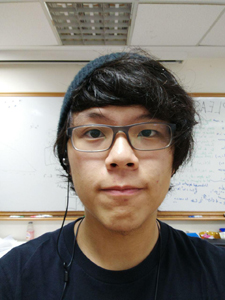
\includegraphics[width=\paperwidth,height=\paperheight]{eldon.png}
  }%
}

\pdfinfo{
  /Title (CS2040S.pdf)
  /Creator (TeX)
  /Producer (pdfTeX 1.40.0)
  /Author (Seamus)
  /Subject (Example)
  /Keywords (pdflatex, latex,pdftex,tex)}

\lstset{language=Java,keywordstyle={\bfseries \color{black}}}

% Turn off header and footer
\pagestyle{empty}

\newenvironment{tightcenter}{%
  \setlength\topsep{0pt}
  \setlength\parskip{0pt}
  \begin{center}
}{%
  \end{center}
}

% redefine section commands to use less space
\makeatletter
\renewcommand{\section}{\@startsection{section}{1}{0mm}%
                                {-1ex plus -.5ex minus -.2ex}%
                                {0.5ex plus .2ex}%x
                                {\normalfont\large\bfseries}}
\renewcommand{\section}{\@startsection{section}{2}{0mm}%
                                {-1explus -.5ex minus -.2ex}%
                                {0.5ex plus .2ex}%
                                {\normalfont\normalsize\bfseries}}
\renewcommand{\subsection}{\@startsection{subsection}{3}{0mm}%
                                {-1ex plus -.5ex minus -.2ex}%
                                {1ex plus .2ex}%
                                {\normalfont\small\bfseries}}%
\renewcommand{\familydefault}{\sfdefault}
\renewcommand\rmdefault{\sfdefault}
% makes nested numbering (e.g. 1.1.1, 1.1.2, etc)
\renewcommand{\labelenumii}{\theenumii}
\renewcommand{\theenumii}{\theenumi.\arabic{enumii}.}
\renewcommand\labelitemii{•}
%  for logical not operator
\renewcommand{\lnot}{\mathord{\sim}}
\renewcommand{\bf}[1]{\textbf{#1}}
\newcommand{\abs}[1]{\vert #1 \vert}
\newcommand{\Mod}[1]{\ \mathrm{mod}\ #1}

\makeatother
\definecolor{myblue}{cmyk}{1,.72,0,.38}
\everymath\expandafter{\the\everymath \color{myblue}}
% Define BibTeX command
\def\BibTeX{{\rm B\kern-.05em{\sc i\kern-.025em b}\kern-.08em
    T\kern-.1667em\lower.7ex\hbox{E}\kern-.125emX}}
\let\iff\leftrightarrow
\let\Iff\Leftrightarrow
\let\then\rightarrow
\let\Then\Rightarrow

% Don't print section numbers
\setcounter{secnumdepth}{0}

\setlength{\parindent}{0pt}
\setlength{\parskip}{0pt plus 0.5ex}
%% this changes all items (enumerate and itemize)
\setlength{\leftmargini}{0.5cm}
\setlength{\leftmarginii}{0.5cm}
\setlist[itemize,1]{leftmargin=2mm,labelindent=1mm,labelsep=1mm}
\setlist[itemize,2]{leftmargin=4mm,labelindent=1mm,labelsep=1mm}

%My Environments
\newtheorem{example}[section]{Example}
% -----------------------------------------------------------------------

\begin{document}
\raggedright
\footnotesize
\begin{multicols*}{4}

% multicol parameters
% These lengths are set only within the two main columns
\setlength{\columnseprule}{0.25pt}
\setlength{\premulticols}{1pt}
\setlength{\postmulticols}{1pt}
\setlength{\multicolsep}{1pt}
\setlength{\columnsep}{2pt}

\begin{center}
    \fbox{%
        \parbox{0.8\linewidth}{\centering \textcolor{black}{
            {\Large\textbf{CS2040S}}
            \\ \normalsize{AY24/25 Sem 2}}
            \\ {\footnotesize \textcolor{myblue}{by ngmh}} 
        }%
    }
\end{center}

\section{Document Distance}
\begin{itemize}
    \item Binary Similarity: Identical texts
    \item Scalar: Number of common words, ratio, etc.
    \item Vector Space Model: Each document is a high-dimensional vector, where dimensions are word frequencies
    \item  To compare 2 words, convert them to vectors, calculate vector norms, dot product, and angle which represents similarity
\end{itemize}

\section{Big-O Notation}
\begin{itemize}
    \item T(n) = Running time on inputs of size n
    \item O = Upper Bound
    \item $\Theta$ = Tight Bound
    \item $\Omega$ = Lower Bound
    \item $T(n) = O(f(n))$ if $T$ grows no faster than $f$
    \item There exists $c > 0$ and $n_0 > 0$ such that for all $n > n_0$, $T(n) \leq cf(n)$
    \item $T(n) = \Omega(f(n))$ if $T$ grows no slower than $f$
    \item There exists $c > 0$ and $n_0 > 0$ such that for all $n > n_0$, $T(n) \geq cf(n)$
    \item $T(n)=\Theta(f(n))$ if and only if $T(n) = O(f(n))$ and $T(n) = \Omega(f(n))s$
    \item If $T(n)$ is a polynomial of degree $k$ then $T(n)=O(n^k)$
    \item If $T(n)=O(f(n))$ and $S(n)=O(g(n))$ then $T(n)+S(n)=O(f(n)+g(n))$ and $T(n) * S(n)=O(f(n)*g(n))$
    \item Sterlings Approximation: $n!\approx \sqrt{2\pi n}(\frac{n}{e})^n$
    \item Appending to String is $O(n)$ in Java
\end{itemize}

\subsection{Solving Recurrences}
\begin{itemize}
    \item Guess and Check using substitution
    \item Drawing recursion tree
    \item Master Theorem
\end{itemize}

\begin{center}
    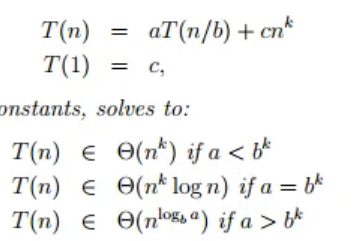
\includegraphics[width=0.7\linewidth]{master.png}    
    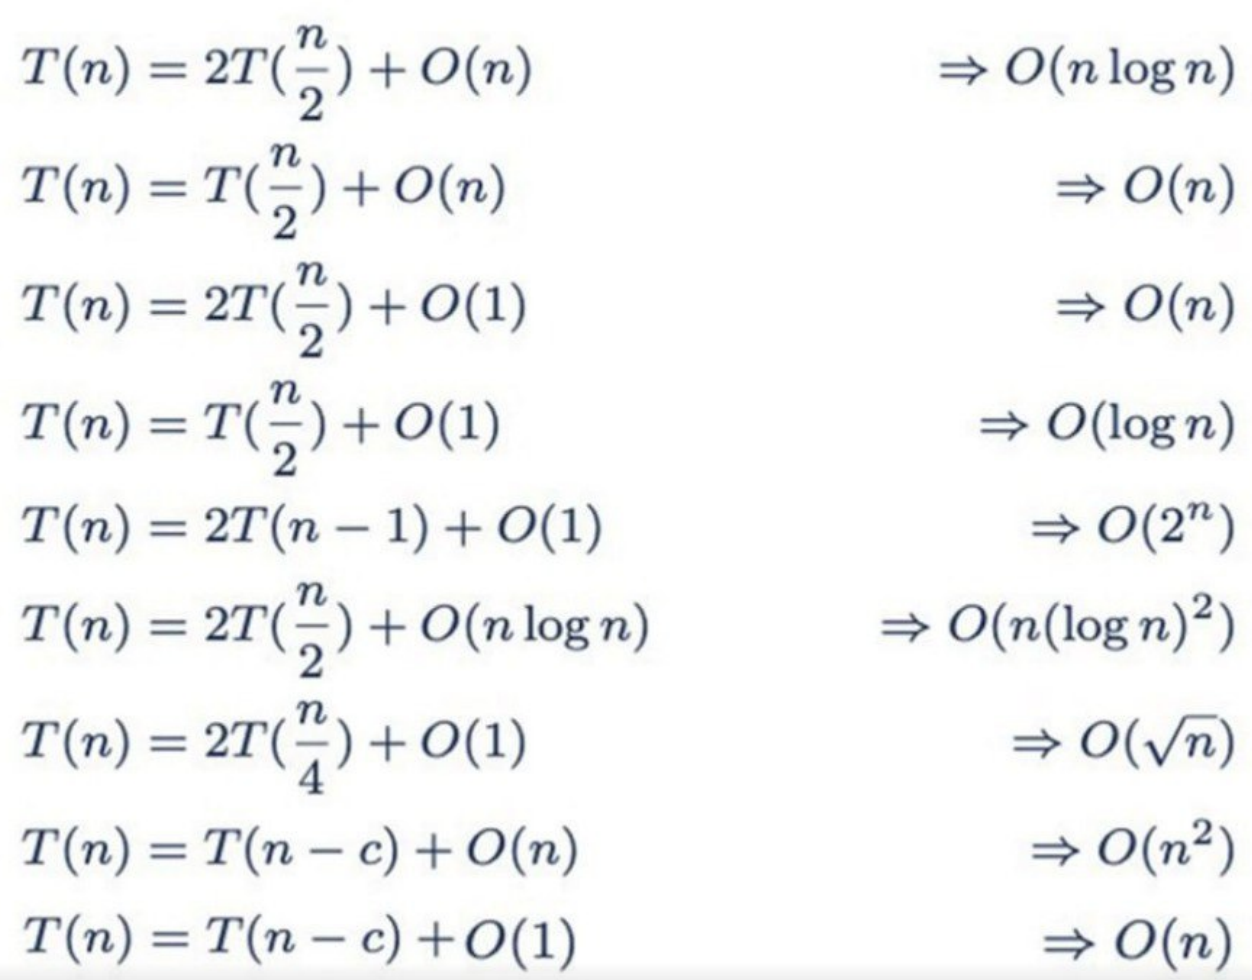
\includegraphics[width=0.9\linewidth]{common.png}    
\end{center}

\begin{center}
\end{center}

\begin{itemize}
    \item Fibonacci: $O(\phi^n)$
    \item Tutorial 2: $T(n) = T(n-1) + T(n-2) + O(1)$
    \begin{itemize}
    \item Guess $T(i)=F(i)-1$
    \item $T(n) = T(n-1) + T(n-2) + 1 = F(n-1) -1 +F(n-2)-1+1=F(n-1)+F(n-2)-1=F(n)-1$
    \end{itemize}
    \item $log(n!)$ tight bound:
    \begin{itemize}
        \item $log(n!)=log(1)+log(2)+...+log(n)\leq nlogn=O(nlogn)$
    \item $log(n!)=log(1)+log(2)+...+log(n) \geq log(n/2)+log(n/2+1)+...+log(n) \geq log(n/2)+log(n/2)+...+log(n/2)=\frac{n}{2}log(\frac{n}{2})=\Omega(n log n))$
    \end{itemize}
    \item $log$ v/s $sqrt$ crap:
    \begin{itemize}
        \item $log(n) < \sqrt{n}$
        \item $log^2(n) < n$
        \item $n^{log(n)} < 2^n$
    \end{itemize}
    \item Chicken Rice Median with QuickSelect: For each level, pivot has $n-1$ bites, and median plate has expected cost of $\frac{1}{n}\cdot n+(1-\frac{1}{n}) \cdot 1 \leq 2$, total is $O(2logn)=O(logn)$ by expectation
\end{itemize}

\subsection{Binary Search}
\begin{itemize}
    \item Preconditions: Condition that is true before running, e.g. Array is sorted and of size n
    \item Invariants: Relationship between variables that is always true, e.g. $A[begin] \leq key \leq A[end]$
    \item Postconditions: Condition that is true after running, e.g. If element is in array: $A[begin] = key$
    \item Can be augmented by binary searching on a monotonic function instead
\end{itemize}
\begin{verbatim}
    int search(A, key, n)
        begin = 0; end = n-1
        while begin < end do:
            mid = begin + (end-begin)/2
            if key <= A[mid]: end = mid
            else: begin = mid+1
        return (A[begin]==key) ? begin : -1
\end{verbatim}

\section{Peak Finding}
\begin{itemize}
    \item Find local maximum in A ($\leq$)
    \item Use divide and conquer to recurse
    \item Invariant: There always exists a peak in the half we recurse on
    \item Correctness: There exists a peak in [begin, end] and every peak in [begin, end] is a peak in [0, n-1]
\end{itemize}
\begin{verbatim}
    FindPeak(A, n)
        if A[n/2] is a peak then return n/2
        else if A[n/2+1] > A[n/2] then
            Search for peak in right half
        else if A[n/2-1] > A[n/2] then
            Search for peak in left half
\end{verbatim}

\subsubsection{Steep Peaks}
\begin{itemize}
    \item Find local maximum in A ($<$)
    \item Cannot use old method, consider case where both sides are equal and we do not know where to recurse
    \item Degenerates to $O(n)$ if we recurse on both half
\end{itemize}

\subsection{2D Peak Finding}
\subsection{Slow Algorithm}
\begin{itemize}
    \item Find global max in each column
    \item Find peak in array of max elements
    \item $O(mn+log(m))$
\end{itemize}

\subsection{Fast Algorithm}
\begin{itemize}
    \item Find peak in array of peaks with lazy evaluation of columns
    \item Find max of middle column
    \item Recurse left / right half by comparing max of adjacent columns
    \item $O(n log m)$
\end{itemize}

\section{Sorting}
\subsection{BogoSort}
\begin{itemize}
    \item Choose a random permutation
    \item Check if sorted
    \item $O(n \cdot n!)$
\end{itemize}

\subsection{BubbleSort}
\begin{itemize}
    \item Repeatedly swap adjacent elements
    \item Best Case: Sorted, $O(n)$
    \item Average / Worst Case: $O(n^2)$
    \item Invariant: At the end of iteration $j$, the biggest $j$ items are correctly sorted in the final $j$ positions of the array
    \item Loop through the whole array $n$ times, swapping any adjacent elements that are out of order
\end{itemize}

\subsection{SelectionSort}
\begin{itemize}
    \item Repeatedly find the minimum element and add it to the prefix
    \item Always $O(n^2)$
    \item Invariant: At the end of iteration $j$, the smallest $j$ items are correctly sorted in the first $j$ positions of the array
    \item Loop through thte whole array $n$ times, finding the minimum and appending it to the prefix by swapping with the end of prefix
\end{itemize}

\subsection{InsertionSort}
\begin{itemize}
    \item Insert the current element into the correct position in the prefix from the back
    \item Best Case: Sorted, $O(n)$
    \item Average / Worst Case: $O(n^2)$
    \item Invariant: At the end of iteration $j$, the first $j$ items in the array are in sorted order
    \item Loop through indexes of the array, each time bubbling the current element from the back down to its correct position
\end{itemize}
\begin{verbatim}
    while (i > 0) and (A[i] > key)
        A[i+1] = A[i]
        i = i-1
    A[i+1] = key
\end{verbatim}

\subsection{MergeSort}
\begin{itemize}
    \item Uses Divide and Conquer
    \item $T(n) = 2T(n/2) + cn$
    \item $logn$ levels, $n$ for each level, $O(nlogn)$
    \item Sort both halves of the array, then merge them together
\end{itemize}

\subsection{QuickSort}
\begin{itemize}
    \item Repeatedly partition the array by a pivot and recurse on both halves
    \item Average Case: $O(n logn)$
    \item Worst Case: $O(n^2)$
\end{itemize}
\begin{itemize}
    \item Maintain a $low$ and $high$ pointer
    \item Non In-Place Partition
    \begin{itemize}
        \item If an element is lower than pivot, add to prefix
        \item If an element is higher than pivot, add to suffix
        \item Invariant: For every $i < low$, $B[i] < pivot$ and for every $j > high$, $B[j] > pivot$
    \end{itemize}
    \item In-Place Partition
    \begin{itemize}
        \item Invariant: $A[high] > pivot$ at the end of each loop
        \item Invariant: For all $i >= high$, $A[i] > pivot$ and for all $1 < j < low$, $A[j] < pivot$
    \end{itemize}
\end{itemize}
    \begin{verbatim}
swap(A[1], A[pIndex])
while (low < high)
    while (A[low] <= p) and (low < high) low++
    while (A[high] > p) and (low < high) high--
    if (low < high) swap(A[low], A[high])
swap(A[l], A[low-1])
    \end{verbatim}
\begin{itemize}
    \item 3-Way Partitioning:
    \begin{itemize}
        \item Two pass: Regular partition, then pack duplicates using high low pointers
        \item One pass: Maintain four regions of array (< pivot, = pivot, in progress, > pivot)
        \item If $A[i] < pivot$, swap with start of = pivot
        \item If $A[i] == pivot$, increment pivot end by 1
        \item If $A[i] > pivot$  swap with start of > pivot
    \end{itemize}
\end{itemize}

\subsection{Paranoid Quicksort}
\begin{itemize}
    \item Partition until a certain partition factor is met (e.g. $9/10$)
    \item Probability of good pivot = $8/10$
    \item $E[Choices] = 1/p = 10/8 < 2$
    \item By expectation, we only have to partition twice
    \item $E[T(n)]=E[T(k)]+E[T(n-k)]+E[Choices](n)\leq E[T(k)]+E[T(n-k)]+2n=O(nlogn)$
    \item $T(n)=T(n/10)+T(9/10)+O(n)=O(n log n)$
\end{itemize}

\subsection{Properties of Sorting Algorithms}
\begin{itemize}
    \item In-Place v/s Not In-Place
    \item MergeSort and QuickSort is not in-place
    \item Stability: Preserving initial order of equal elements
    \item SelectionSort and QuickSort are not stable due to swaps
    \item Insertion and Bubble Complexity: Swap first and last element
\end{itemize}

\subsection{QuickSelect}
\begin{itemize}
    \item Select the $k^{th}$ smallest element in an unsorted array
    \item Randomly partition, with paranoia
    \item Recurse only on correct half
    \item $E[T(n)] \leq E[T(9n/10)]+E[Partitions](n) \leq E[T(9n/10)]+2n \leq O(n)$
\end{itemize}

\subsection{Trees}
\begin{itemize}
    \item Binary Search Tree: Keys in left < Key < Keys in right
    \item Height: $0$ at leaf, increases by $1$ for each parent, maximum of children
    \item Insertion: Traverse until respective child does not exist on node and just add
    \item In-Order: LSR; Pre-Order: SLR; Post-Order: LRS
    \item Level-Order: Greatest height to lowest Height, from left to right
    \item Successor:
    \begin{itemize}
        \item Search for key
        \item If $result > key$ return $result$
        \item If $result \leq key$ search for $succesor(result)$
        \item $successor():$
    \end{itemize}
\end{itemize}
    \begin{verbatim}
    if (righTree != null) return rightTree.min()
    TreeNode parent = parentTree
    TreeNode child = this
    while parent != null && child == parent.right
        child = parent
        parent = child.parentTree
    return parent
    \end{verbatim}
\begin{itemize}
    \item Deletion:
    \begin{itemize}
        \item 1 Child: Remove v, Connect child(v) to parent(v)
        \item 2 Children: Delete successor and replace node with it
    \end{itemize}
\end{itemize}

\subsection{AVL Trees}
\begin{itemize}
    \item Balanced Tree: $h=O(logn)$
    \item Height Balanced Tree: $|v.left.height - v.right.height| \leq 1$, has at most $h < 2log(n)$ nodes and at least $n > 2^{h/2}$
    \item Weight Balanced Tree: $v.left.w, v.right.w \leq \alpha \ v.w$
    \item Height / Weight Balanced implies Balanced but not the other way round
    \item Maximally Imbalanced: AVL tree with minimum possible number of nodes given its height
    \item Left / Right Heavy: Which child has larger height
    \item Rotations
    \begin{itemize}
        \item Direction is where root of subtree goes
        \item Requires a child opposite of rotation direction
        \item v Left
        Heavy: Check Left child:
        \begin{itemize}
            \item Balanced: Right-Rotate(v)
            \item Left Heavy: Right-Rotate(v)
            \item Right Heavy: Left-Rotate(v.left), Right-Rotate(v)
        \end{itemize}
        \item v Right
        Heavy, Check Right child:
        \begin{itemize}
            \item Balanced: Left-Rotate(v)
            \item Left Heavy: Right-Rotate(v.right), Left-Rotate(v)
            \item Right Heavy: Left-Rotate(v)
        \end{itemize}
        \item Basically if middle heavy rotate child away from middle first before rotating root of subtree
        \item Credits to Way Yan (for tracing):
    \end{itemize}
\end{itemize}
\begin{center}
    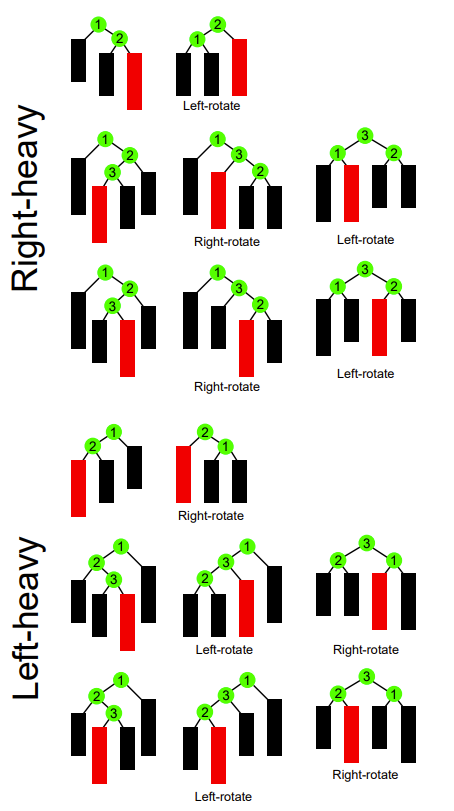
\includegraphics[width=0.7\linewidth]{rotation.png}    
\end{center}
\begin{itemize}
    \item Insertion:
    \begin{itemize}
        \item Only need to fix lowest unbalanced node after deletion, with at most two rotations
        \item Since rotating reduces height by 1, the height after rotation will be correct
    \end{itemize}
    \item Deletion
    \begin{itemize}
        \item Swap node with ancestor if it has 2 children
        \item Delete node from tree, reconnecting children
        \item Recurse upwards and rotate if needed, up to $O(logn)$ needed
        \item Since height after rotation might be less than height before deletion
    \end{itemize}
    \item Potential Modification: Only store difference in height from parent
\end{itemize}

\subsection{Scapegoat Tree}
\begin{itemize}
    \item 2/3 Weight-Balanced tree
    \item Unbalanced: Child has more than $2/3$ of the total subtree weight
    \item Rebuild tree at highest unbalanced node
\end{itemize}

\subsection{Augmenting Data Structures}
\begin{itemize}
    \item Choose underlying data structure, Additional information, Maintain updates of information, Develop new operations
    \item Order statistics: Rank and Select, use subtree size information to determine where to recurse
    \item Counting Inversions: At each index, the inversion count is tree size minus rank of current element
\end{itemize}

\subsection{Order Statistic Trees}
\begin{itemize}
    \item Augment with weight of each node
    \item $select(k)$: Finds node with rank $k$
    \begin{verbatim}
    rank = left.weight+1
    if k == rank return v
    if k < rank return left.select(k)
    if k > rank return right.select(k-rank)
    \end{verbatim}
    \item $rank(node)$ Computes rank of a node $v$
    \begin{verbatim}
    rank = left.weight+1
    while node != null
        if node == par.right
            rank += par.left.weight + 1
        node = par
    return rank
    \end{verbatim}
\end{itemize}

\section{Tries}
\begin{itemize}
    \item Store letters in nodes
    \item Words are represented as paths from root to leaf
    \item Use special mark for terminal node / character
\end{itemize}

\section{$(a,b)$-trees}
\begin{itemize}
    \item Restriction: $2 \leq a \leq (b+1)/2$.
    \item Rule 1: $(a,b)$-child policy
    \begin{itemize}
        \item Root node must have between $1$ and $b-1$ keys
        \item Internal / Leaf node must have between $a-1$ and $b-1$ keys
        \item Leaf node has no children
    \end{itemize}
    \item Rule 2: Key ranges
    \begin{itemize}
        \item A non-leaf node has one more child than number of keys
        \item Each subtree has a key range
    \end{itemize}
    \item Rule 3: Leaf depth
    \begin{itemize}
        \item All leaf nodes must be at the same depth
    \end{itemize}
    \item B-Tree: $(B, 2B)$-tree, where $B$ is block size of a storage device
    \item Min / Max Height: $O(log_bn)$, $O(log_an)+1$
    \item Searching: At each node, binary search for corresponding key range to recurse on, taking $O(log_2b \cdot log_an)=O(logn)$ time
    \item Insertion:
    \begin{itemize}
        \item Insert at leaf node
        \item Redistribute keys if it violates size limit by performing a split
        \begin{itemize}
            \item Find median key $v_m$
            \item Separate all keys $\leq v_m$ to make a new node $y$
            \item Give $y$ the final child from the left of $v_m$
            \item Insert $v_m$ into parent
            \item Connect $v_m$ to the new node $y$ we created
            \item Recurse upwards if needed
        \end{itemize}
        \item Works as LHS $=\lfloor(b-1)/2)\rfloor=\lfloor a - 1/2 \rfloor$ and RHS $= \lceil (b-1)/2\rceil =\lceil a-1/2 \rceil$, and $\lfloor a-1/2 \rfloor \geq a-1$
        \item Proactive: Preemptively split any node at full capacity ($b-1$) during search phase
        \begin{itemize}
            \item Must have $b \geq 2a$
            \item After split, left sibling has $\lfloor (b-2)/2 \rfloor=\lfloor b/2 \rfloor-1$ keys
            \item After splitting, it must have $\geq a-1$ keys
            \item $\lfloor b/2 \rfloor -1 \geq a-1$, $\lfloor b/2 \rfloor \geq a$, $b \geq 2a$
        \end{itemize}
        \item Passive: Perform insertion first then check parent for violation and recurse
    \end{itemize}
    \item Deletion:
    \begin{itemize}
        \item Search for key, then delete from keylist
        \item However, number of keys might fall below $a-1$
        \item Suppose $z$ is offending, and $y$ is smallest sibling
        \item Merge with sibling if necessary
        \item $y+z < b-1$:
        \begin{itemize}
            \item In parent, delete key $v$ separating siblings
            \item Add $v$ to keylist of $y$
            \item In $y$, merge in $z$'s keylist and treelist
            \item Remove $z$
        \end{itemize}
        \item $y+z \geq b-1$
        \begin{itemize}
            \item Perform sharing by $merge(y, z)$ followed by splitting merged node
            \item By definition of $(a,b)$-trees, they will have at least $b+1$ keys after taking one from the parent
            \item LHS has $\lfloor (b+1)/2 \rfloor \geq a$, RHS has $\lceil (b+1)/2 \rceil \geq a$
        \end{itemize}
        \item Proactive: Preemptively merge and share any node at minimal capacity ($a-1$) during search phase
        \item Passive: Delete first then check parent for violation and recurse
        \item If deleting a key results in orphaned children, swap out key with a leaf node key (successor) before deleting
    \end{itemize}
\end{itemize}

\begin{center}
    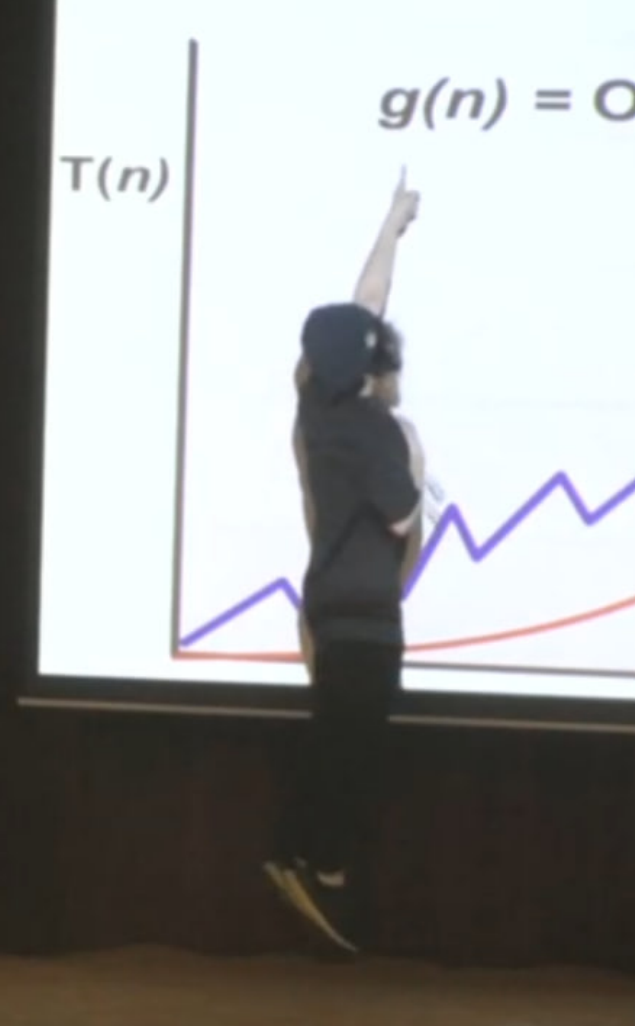
\includegraphics[width=0.5\linewidth]{jump.png}    
\end{center}

\begin{center}
    \begin{tabular}{lll}
    \raisebox{-.5\height}{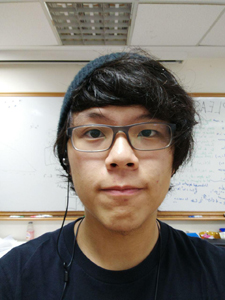
\includegraphics[scale=0.5]{eldon.png}} & pls give me A+ eldon thanks \\
    \end{tabular}
\end{center}

\end{multicols*}

\end{document}